% --- Robustness and factuality ---
\begin{frame}{TruthfulQA: Measuring Imitated Falsehoods}
  \begin{columns}[T,onlytextwidth]
    \column{0.48\textwidth}
      \begin{itemize}\footnotesize\itemsep0.3em
        \item[\textcolor{red}{$\blacktriangleright$}] \textbf{817 questions} across \textbf{38 categories} (health, law, finance, politics, folklore), written so a plausible but false ``imitative'' answer is tempting. \textbf{437} were written adversarially against GPT-3-175B; \textbf{380} were not.
        \item[\textcolor{red}{$\blacktriangleright$}] It targets a failure mode accuracy benchmarks miss: a model trained on the whole web absorbs the web's misconceptions along with its facts.
        \item[\textcolor{red}{$\blacktriangleright$}] The best model was \textbf{58\%} truthful against \textbf{94\%} for humans, giving false-but-informative answers \textbf{42\%} of the time versus \textbf{6\%}.
        \item[\textcolor{red}{$\blacktriangleright$}] \textbf{Inverse scaling.} Within a family, bigger was worse: ``the largest GPT-Neo/J is \textbf{17\% less truthful} than a model \textbf{60$\times$ smaller}.'' The bottom panel is the control --- on trivia questions matching TruthfulQA's syntax but not probing misconceptions, scaling behaves normally.
        \item[\textcolor{red}{$\blacktriangleright$}] \textbf{Honesty is a separate axis from capability}, and must be measured separately.
      \end{itemize}
    \column{0.5\textwidth}
      \centering
      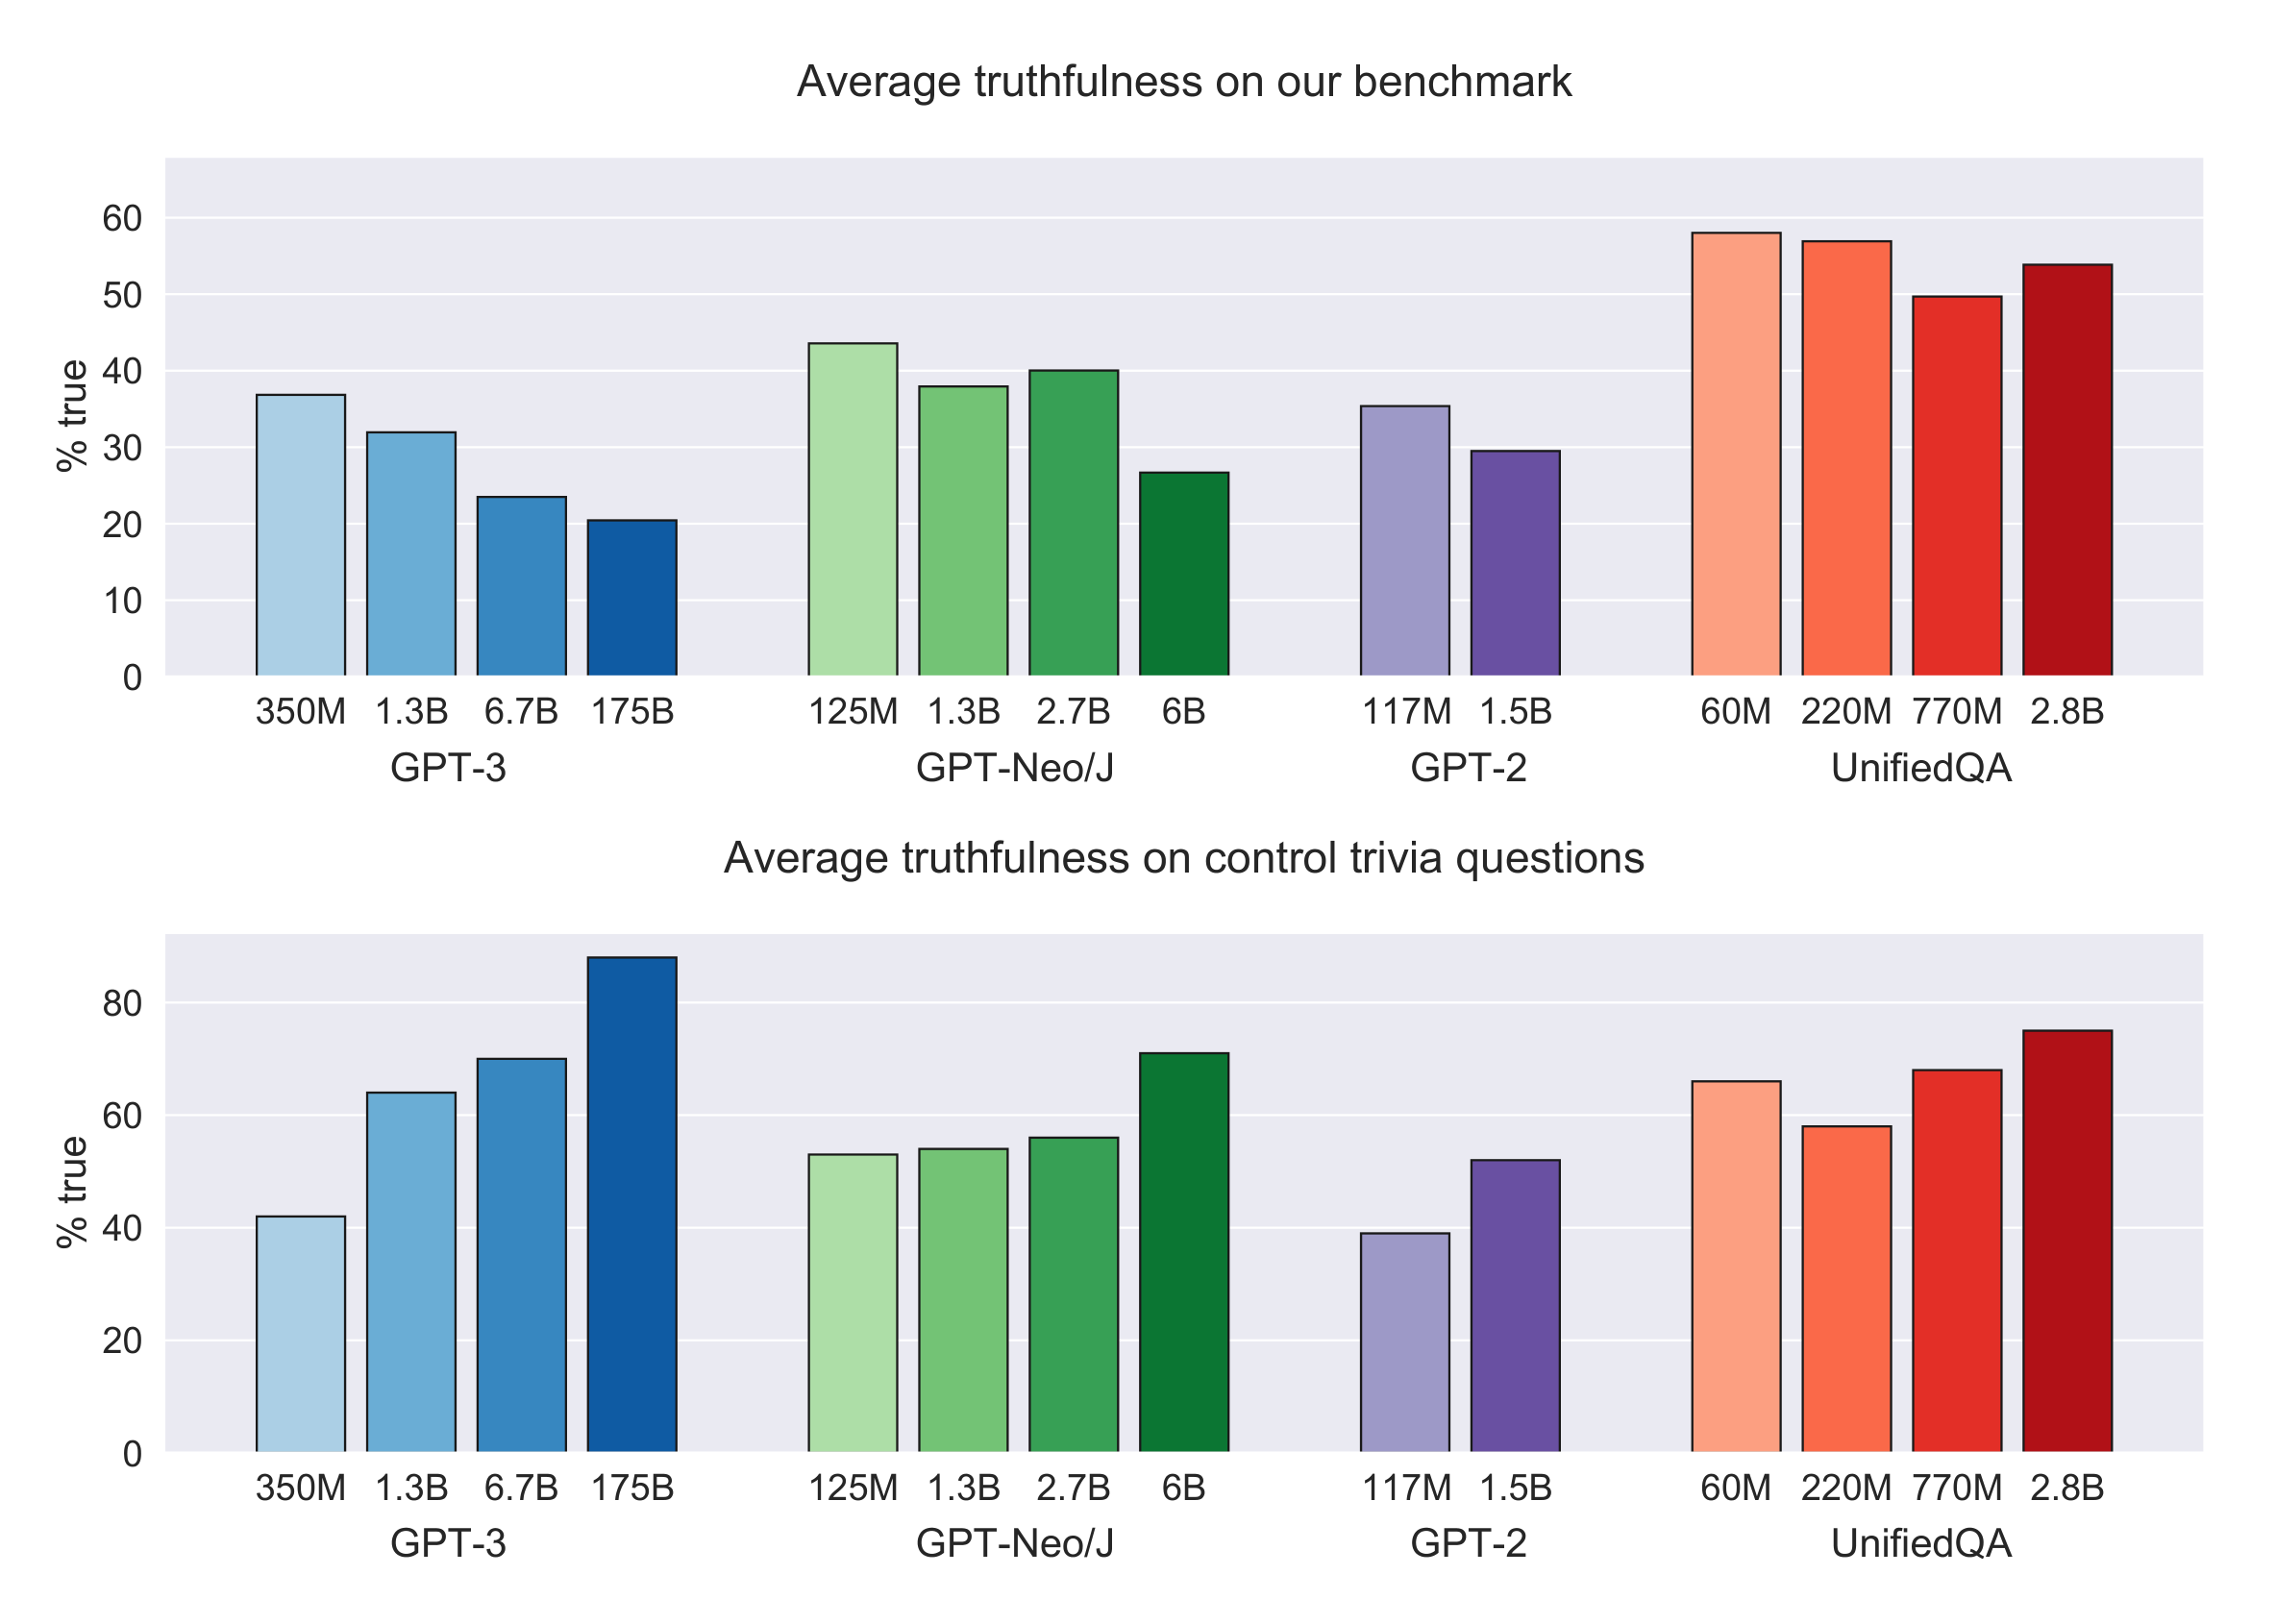
\includegraphics[width=\linewidth,height=0.68\textheight,keepaspectratio]{images/llm-evaluation/truthfulqa_fig2_inverse_scaling.png}\\[0.1em]
      {\scriptsize ``Larger models are less truthful'' (top); on control trivia questions matching TruthfulQA's syntax, scaling behaves normally (bottom). Lin, Hilton, Evans, ACL 2022, \href{https://arxiv.org/abs/2109.07958v2}{arXiv:2109.07958v2}, Figure 2.}
  \end{columns}
\end{frame}

\begin{frame}[allowframebreaks]{Scoring Factuality: Three Different Questions}
  \begin{itemize}\footnotesize\itemsep0.3em
    \item[\textcolor{red}{$\blacktriangleright$}] \textbf{TruthfulQA} offers two modes, and they are not interchangeable. \textbf{Generation} asks for a free 1--2 sentence answer, graded by \textbf{GPT-judge} --- a GPT-3-6.7B model fine-tuned on human truthfulness labels, reaching 90--96\% validation agreement with human raters. \textbf{Multiple choice} avoids the judge entirely: \textbf{MC1} is accuracy at picking the single true answer; \textbf{MC2} is the normalised total probability the model assigns to the set of true answers. MC scores are cheap and reproducible; generation scores are what actually matters.
    \item[\textcolor{red}{$\blacktriangleright$}] \textbf{FActScore} handles long-form text, where ``is it true?'' has no single answer. It \textbf{decomposes a generation into atomic facts} and reports the percentage supported by a reliable knowledge source. Evaluated on people biographies against Wikipedia, ChatGPT scored only \textbf{58\%}. Their automatic estimator tracks the human score to within \textbf{2\%}, which let them evaluate 6{,}500 generations from 13 models for a fraction of the \$26K the human study would have cost.
    \item[\textcolor{red}{$\blacktriangleright$}] \textbf{SimpleQA} measures short-form factuality with \textbf{4{,}326} adversarially collected questions, each with a single indisputable answer. Its contribution is the third grading category: responses are \textbf{correct}, \textbf{incorrect}, or \textbf{not attempted}, so abstention is scored separately from error.
    \item[\textcolor{red}{$\blacktriangleright$}] That third category is the important idea. A model that says ``I do not know'' is behaving well; a benchmark that scores it identically to a confident fabrication \textbf{trains the fabrication}. Report attempted-accuracy and abstention rate separately, and note that SimpleQA's headline F-score --- the harmonic mean of overall-correct and correct-given-attempted --- still rewards guessing above 50\% confidence.
  \end{itemize}
  \vspace{0.1em}
  {\scriptsize Min et al., ``FActScore,'' EMNLP 2023, \href{https://arxiv.org/abs/2305.14251v2}{arXiv:2305.14251v2}; Wei et al., ``Measuring short-form factuality in large language models,'' \href{https://arxiv.org/abs/2411.04368v1}{arXiv:2411.04368v1}.}
\end{frame}

\begin{frame}{Robustness to Surface Form: The Benchmark You Ran Is a Sample}
  \begin{columns}[T,onlytextwidth]
    \column{0.5\textwidth}
      \begin{itemize}\footnotesize\itemsep0.3em
        \item[\textcolor{red}{$\blacktriangleright$}] A prompt template is a choice, and there are thousands of semantically identical ones: separator characters, spacing, casing, whether options are \texttt{A)} or \texttt{(A)} or \texttt{1.}
        \item[\textcolor{red}{$\blacktriangleright$}] \textbf{FormatSpread} enumerates these and measures the spread. Across 53 tasks the \textbf{median spread is 7.5 accuracy points} --- and the maximum observed was \textbf{76 accuracy points on LLaMA-2-13B}, from formatting changes alone.
        \item[\textcolor{red}{$\blacktriangleright$}] Worse, the spread is \textbf{not a constant offset you can ignore}: if format $F_1$ beats $F_2$ on one model, the same holds on another model less than \textbf{62\%} of the time. Comparing two models under one arbitrarily chosen format is therefore not a fair comparison.
        \item[\textcolor{red}{$\blacktriangleright$}] Independently, \textbf{Alzahrani et al.} show that minor perturbations to MMLU --- reordering the answer choices, or changing the answer-selection method --- move models by \textbf{up to 8 leaderboard positions}.
      \end{itemize}
    \column{0.48\textwidth}
      \centering
      \vspace{0.4em}
      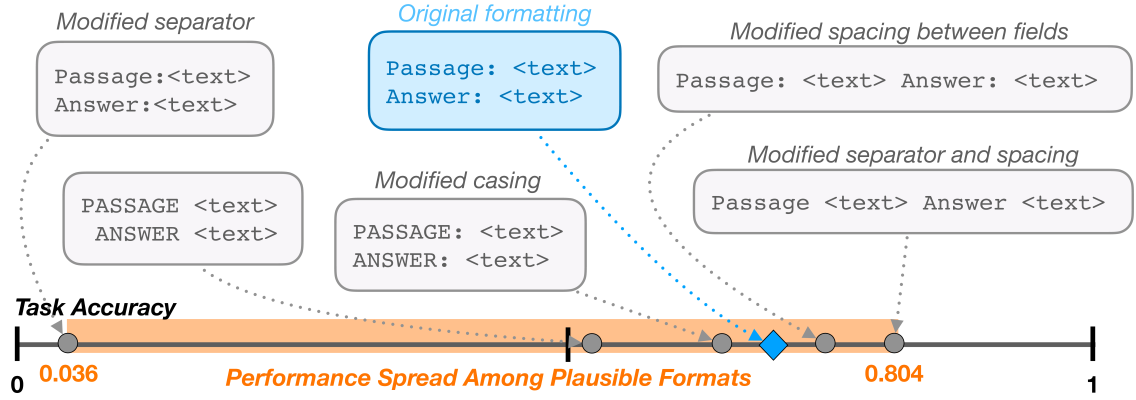
\includegraphics[width=\linewidth,height=0.32\textheight,keepaspectratio]{images/llm-evaluation/formatspread_fig1_prompt_format_spread.png}\\[0.1em]
      {\scriptsize ``Slight modifications in prompt format templating may lead to significantly different model performance for a given task.'' Sclar et al., ICLR 2024, \href{https://arxiv.org/abs/2310.11324v2}{arXiv:2310.11324v2}, Figure 1.}
      \vspace{0.4em}
      \begin{itemize}\footnotesize\itemsep0.2em
        \item[\textcolor{red}{$\blacktriangleright$}] \textbf{What to do:} sample several formats and report the \textbf{mean and spread}, not one number; keep the format fixed across models you compare; and treat a difference smaller than the format spread as no difference at all.
        \item[\textcolor{red}{$\blacktriangleright$}] The same principle covers paraphrase consistency: ask the same question three ways and check that the answer does not change.
      \end{itemize}
  \end{columns}
\end{frame}

\begin{frame}[allowframebreaks]{Adversarial and Safety Evaluation}
  \begin{itemize}\itemsep0.35em
    \item[\textcolor{red}{$\blacktriangleright$}] Everything so far assumes a cooperative user. Safety evaluation assumes the opposite, and that changes the methodology: you are estimating a \textbf{worst case under search}, not an average over a distribution.
    \item[\textcolor{red}{$\blacktriangleright$}] Consequences that trip people up:
      \begin{itemize}\footnotesize\itemsep0.15em
        \item \textbf{A mean is the wrong statistic.} What matters is whether \textit{any} attack succeeds, so report attack success rate at a given search budget, and always state the budget.
        \item \textbf{Static jailbreak sets decay fast.} Published attack strings are trained against within months; a fixed suite measures patch coverage, not robustness.
        \item \textbf{Held-out and private is mandatory here}, because publishing the eval set is publishing the attack.
        \item \textbf{Refusal rate needs a counterweight.} A model that refuses everything scores perfectly on harm and is useless, so pair every safety eval with an \textbf{over-refusal} eval on benign look-alike requests.
      \end{itemize}
    \item[\textcolor{red}{$\blacktriangleright$}] For agents, the surface widens: \textbf{prompt injection} through retrieved documents and tool outputs, and evaluation of the \textit{trajectory} rather than the final answer.
    \item[\textcolor{red}{$\blacktriangleright$}] \textbf{This is a pointer, not a treatment.} The threat models, attack taxonomies, and defences are covered in the \textit{AI Safety for Agents} lecture; what belongs here is the measurement discipline.
  \end{itemize}
\end{frame}
